\documentclass[twocolumn]{article}
\usepackage{sonar}
%\usepackage{graphicx}


\begin{document}

\section{Random under sonar theme}

\subsection{Deep sea from Wikipedia}
The deep sea 1 21 or deep layer[1] is the lowest layer in the ocean, existing below the thermocline and above the seabed, at a depth of 1000 fathoms (1800 m) or more. Little or no light penetrates this part of the ocean, and most of the organisms that live there rely for subsistence on falling organic matter produced in the photic zone. For this reason, scientists once assumed that life would be sparse in the deep ocean, but virtually every probe has revealed that, on the contrary, life is abundant in the deep ocean.

    From the time of Pliny until the late nineteenth century...humans believed there was no life in the deep. It took a historic expedition in the ship Challenger between 1872 and 1876 to prove Pliny wrong; its deep-sea dredges and trawls brought up living things from all depths that could be reached. Yet even in the twentieth century scientists continued to imagine that life at great depth was insubstantial, or somehow inconsequential. The eternal dark, the almost inconceivable pressure, and the extreme cold that exist below one thousand meters were, they thought, so forbidding as to have all but extinguished life. The reverse is in fact true....(Below 200 meters) lies the largest habitat on earth.

 See also:
\begin{itemize}
\item Deep sea fish
\item Deep ocean water
\item Submarine landslide
\item \emph{The Blue Planet}
\end{itemize}

There are a number of species that do not primarily rely upon dissolved organic matter for their food and these are found at hydrothermal vents. One example is the symbiotic relationship between the tube worm Riftia and chemosynthetic bacteria. It is this chemosynthesis that supports the complex communities that can be found around hydrothermal vents. These complex communities are one of the few ecosystems on the planet that do not rely upon sunlight for their supply of energy.


\section{Sonar}
Sonar (originally an acronym for SOund Navigation And Ranging) is a technique that uses sound propagation (usually underwater, as in submarine navigation) to navigate, communicate with or detect objects on or under the surface of the water, such as other vessels. Two types of technology share the name "sonar": passive sonar is essentially listening for the sound made by vessels; active sonar is emitting pulses of sounds and listening for echoes. Sonar may be used as a means of acoustic location and of measurement of the echo characteristics of "targets" in the water. Acoustic location in air was used before the introduction of radar. Sonar may also be used in air for robot navigation. The term sonar is also used for the equipment used to generate and receive the sound. The acoustic frequencies used in sonar systems vary from very low (infrasonic) to extremely high (ultrasonic).

Figure\ref{fig:sample} shows a sonar image of shipwreck of the Soviet Navy minesweeper T-297, formerly the Latvian Virsaitis in Estonian waters 20 km from Keri island.
\begin{figure}
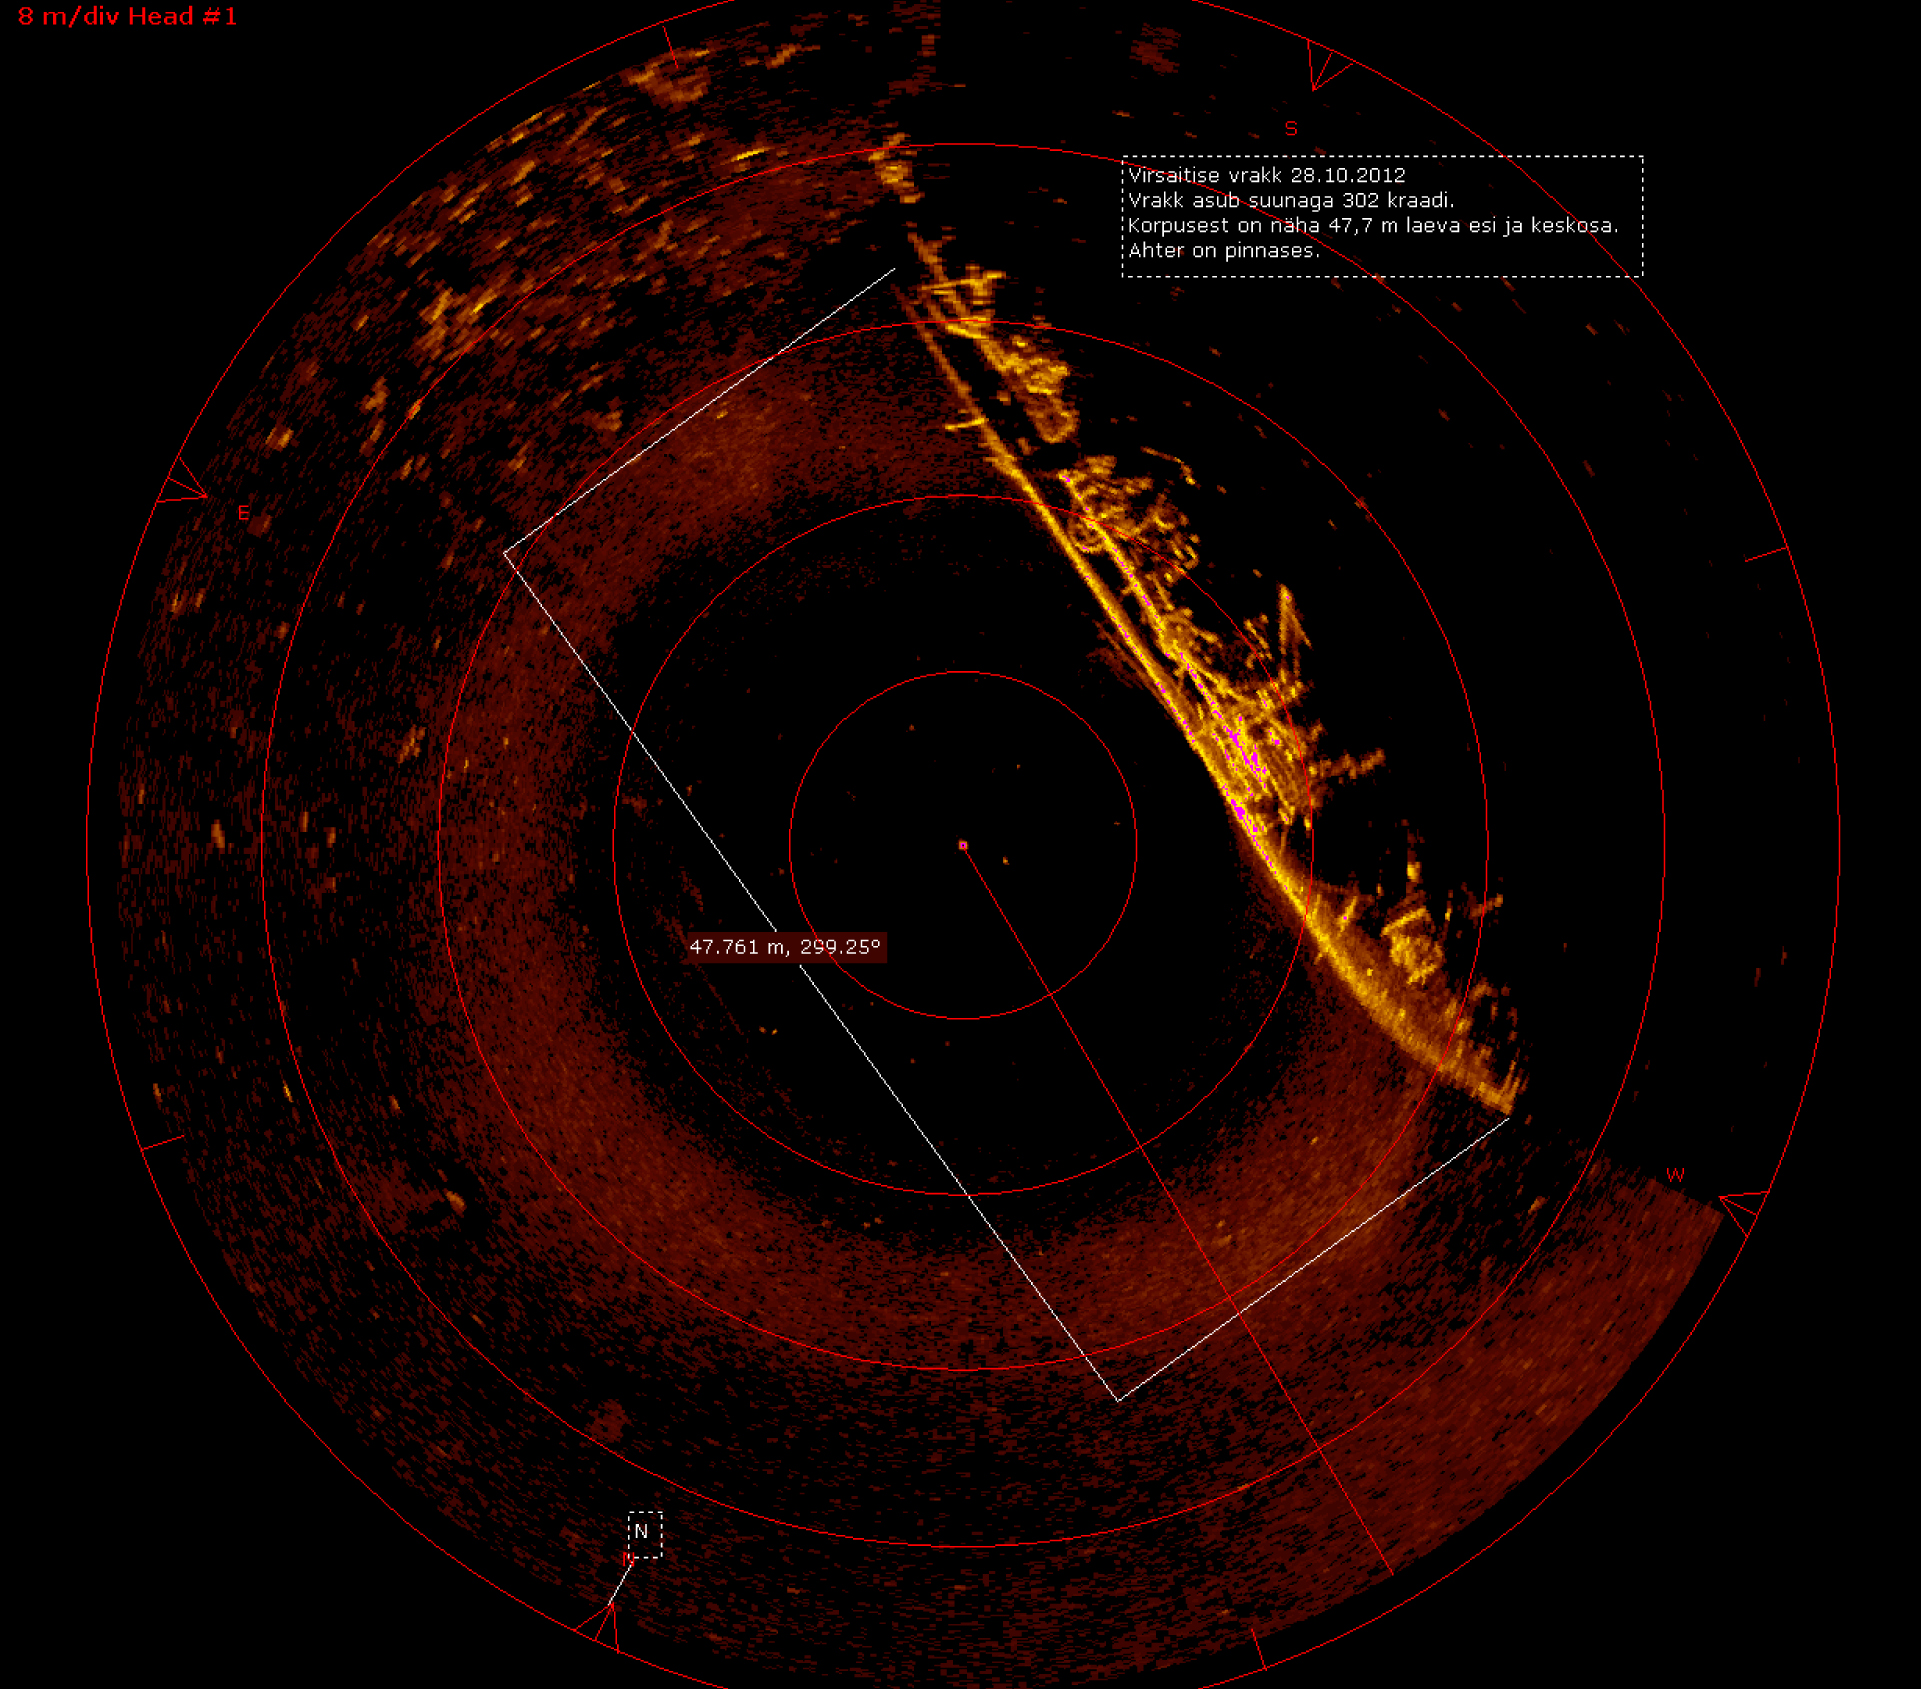
\includegraphics[scale=0.45]{pics/sonarWikiPic}
\caption{\label{fig:sample}Taken from wikipedia: \emph{A sonar image of the shipwreck of the Latvian Navy ship Virsaitis.}}
\end{figure}


\subsection{Effect of sonar on marine life}
Sonars have been developed that can be used to characterise the sea bottom (fig\ref{fig:sample2}) into, for example, mud, sand, and gravel. Relatively simple sonars such as echo sounders can be promoted to seafloor classification systems via add-on modules, converting echo parameters into sediment type. Different algorithms exist, but they are all based on changes in the energy or shape of the reflected sounder pings. Advanced substrate classification analysis can be achieved using calibrated (scientific) echosounders and parametric or fuzzy-logic analysis of the acoustic data. An equation at eq\ref{eq:1}
\begin{figure}
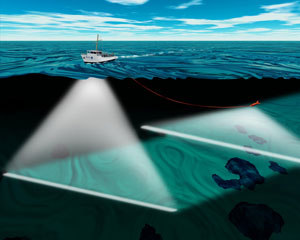
\includegraphics[scale=0.4]{pics/seabedWikiPic}
\caption{\label{fig:sample2}Taken from wikipedia: \emph{Graphic depicting NOAA hydrographic survey ship conducting multibeam and side scan sonar operations}}
\end{figure}

Active sonar limitations at initial detection (no $\alpha$):
\begin{equation}
  \label{eq:1}
SL - 2TL + TS - (NL-DI) = DT
\end{equation}



\end{document}

